\documentclass[11pt, a4paper]{article}
\usepackage[margin=1in]{geometry}
\usepackage{graphicx}
\usepackage{float}
\usepackage{hyperref}

\hypersetup{
    colorlinks=true,
    linkcolor=blue,
    urlcolor=cyan
}

\makeatletter
\renewcommand\paragraph{\@startsection{paragraph}{4}{\z@}%
            {-2.5ex\@plus -1ex \@minus -.25ex}%
            {1.25ex \@plus .25ex}%
            {\normalfont\normalsize\bfseries}}
\makeatother
\setcounter{secnumdepth}{4}
\setcounter{tocdepth}{4}

\title{Module5}
\author{Puru Vaish}
\date{\today}

\begin{document}
\maketitle

\section{Lecture One}
\subsection{Boolean Algebra}
\subsubsection{Basic}
\begin{figure}[H]
    \centering
    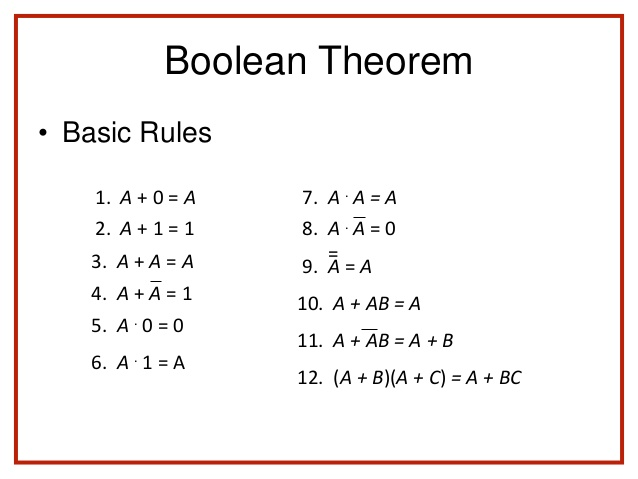
\includegraphics[width =\textwidth]{Pictures/BooleanAlgebra.jpg}
    \caption{Basic Rules}
\end{figure}
\subsubsection{XOR}
A xor B = A.$\overline{B}$ + $\overline{A}$.B
\subsubsection{De Morgan}
$\overline{(A + B)}=\overline{A}.\overline{B}$\newline
$\overline{(A.B)}=\overline{A}+\overline{B}$

This important for NAND/NOR only circuit conversions.

\subsection{SOP}
SOP: Sum of Products (A.B no A.(B+C) like terms)
This is represented using F(A,B,C,D) = A.B + C.D and so on.

\subsection{Medium Scale Integration}
\begin{enumerate}
    \item Multiplexer
    \item Demultiplexer
    \item Decoder
    \item Priority Encoder
\end{enumerate}

\subsubsection{Multiplexer}
\begin{figure}
    \centering
    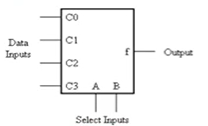
\includegraphics{Pictures/Multiplexer.png}
    \caption{Multiplexer}
\end{figure}
Using the Selected Input values, a particular Data Input is passed into the Output.
The internal is as follows:
\begin{figure}[H]
    \centering
    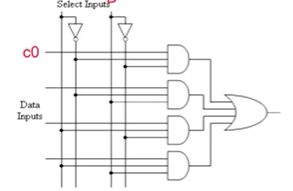
\includegraphics{Pictures/MultiplexerInternal.png}
    \caption{Internal}
\end{figure}

As we can see the two selected inputs A,B can be 4 possible values, and this is used to selected the Data Input, or sometimes the bit from the data input.

Implementation of logical circuits using Multiplexors:
\begin{enumerate}
    \item Set $c_1$, $c_2$ and so on depending on selected inputs. $c_n$ data inputs exist where $n=2^{no. of selected inputs}$.
    \item \textbf{NOT Gate using 2:1 Mux}
    \begin{enumerate}
        \item Set $c_1$ to 1 and $c_2$ to 0.
        \item If Selected Input (x) is 0, 1 is Output
        \item else if $x=1$, $0$ is output.
    \end{enumerate}
    \item \textbf{OR GATE using 2:1}
    \begin{enumerate}
        \item OR Gate has two inputs, so one of the inputs is used as selected input, and the other is used as data input $c_1$
        \item Set $c_2$ to 1.
        \begin{figure}[H]
            \centering
            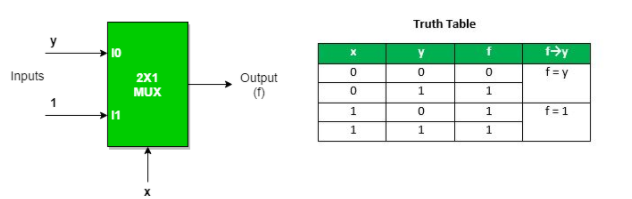
\includegraphics[width = \textwidth]{Pictures/MakingLogicUsingMux.png}
            \caption{OR GATE}
        \end{figure}
    \end{enumerate}
    \item For more such examples: \href{https://www.geeksforgeeks.org/multiplexers-in-digital-logic/}{Geeks For Geeks}
    \item Example:
    \begin{figure}[H]
        \centering
       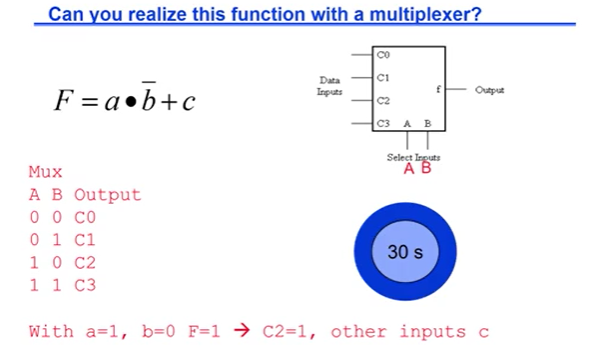
\includegraphics{Pictures/MakingLogicExc.png}
        \caption{Example}
    \end{figure}
\end{enumerate}
\subsubsection{Demultiplexor}
This is the inverse of multiplexor
\begin{figure}[H]
    \centering
    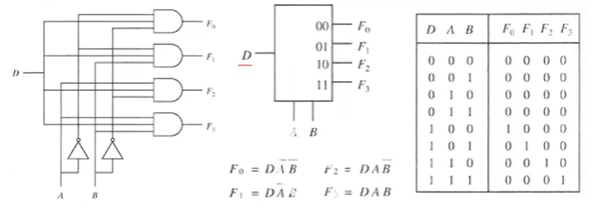
\includegraphics{Pictures/Demultiplexor.png}
    \caption{Demultiplexor}
\end{figure}
SO basically it maps the selected inputs to the data input the represent, $(0,0)$ -> $c_0$ when there is data D present.

\subsubsection{Decoder}
\begin{enumerate}
    \item The selected inputs S determines which output is 1 (all others are 0). So, for three selected inputs there are 8 outputs, $2^{3}$.
    \item m<nr> is minterm, which means m0 -> 00 in a 2 selected input decoder and m3 corresponds to 11 output.
    \item A decoder can also have an enable input. When disabled all outputs are 0.
    \item It can be used to extend the address range of a memory bank.
    \item The hardware internals is the same as demultiplexor, so it is the use under which they are which changes there name.
\end{enumerate}

\subsubsection{Priority Encoder}
\begin{enumerate}
    \item MSB to the first 1 is noted, other bits are not cared for. Depending on the position of the first 1, an 8->3 map is defined to give a prioroty rank, hence if MSB 7 is 1 -> 111, and so on.
    \item A prioroty encoder can be used fot arbitration between devices that compete for the same resource.
\end{enumerate}

\subsection{Methods of Solving Logical Circuits}
\begin{enumerate}
    \item Algebraic Reduction - Very Long, need to bring $B.1 = B.(C+\overline{C})$ which is rather un-intuitive, \textbf{but a law}
    \item Karnough Maps
    \item Writing the truth table and miraculously finding the solutions in 1 sec. Rarely effective like that.
\end{enumerate}

\subsubsection{Karnaugh Maps}
Mostly A-Level, but little new thing:
\paragraph{Don't Care Symbol}
For Example, we only care about the outputs of 8 different states where 4 are noted as 1 and rest 4 are 0. The same thing in a 16 input setting will result in 8 states we don't care about. So, when solving a Karnoguh map, we can see them as 1 or 0, and depending on the one giving a better minimum we draw up our circuit.
\begin{figure}[H]
    \centering
    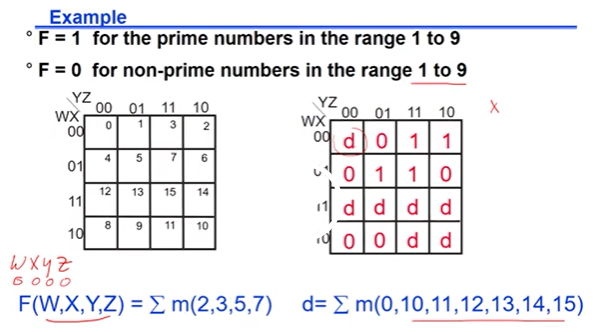
\includegraphics[width = \textwidth]{Pictures/KarnaughMap with dont care.png}
    \caption{Karnaugh Map with don't care Example}
\end{figure}
Final Result = $\overline{X}.Y + X.Z$

\subsection{Combination Logic and Sequential Logic}

\subsubsection{Latch}
\paragraph{SR Latch with NORs}
A Level stuff
S=1, R=1 is illegal, due to race conditions, unstable circuit, pulse racing for output, not predictable.

\begin{figure}[H]
    \centering
    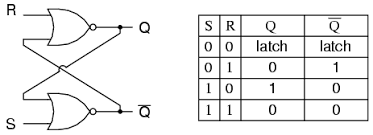
\includegraphics[width = \textwidth]{Pictures/SR-Latch.png}
    \caption{SR Latch}
\end{figure}

\paragraph{Truth Table Remember Trick}
\begin{enumerate}
    \item S (the top one) is Set, hence sets Q = 1
    \item R (lower) is Reset, hence sets Q = 0,
    \item If both are 0, then no change,
    \item If trying to both, then illegal.
\end{enumerate}


\paragraph{D-Latch (Data Latches)}
\begin{enumerate}
    \item Has two inputs: Control, Data (C,D) and output Q
    \item C=0, Q=Q, last state, no change on D
    \item C=1, Q=D, Q now equal to D
    \item This acts like a Latch
    \item Using Karnaugh -> $C.D + \overline{C}.D$
    \item But this is not exactly correct, due to the feedback in the circuit
    \item Due to the feedback, when D=1, and C transistions from 1 to 0, Q should remain 1, but, it is not the case, \textbf{Due to timing differences, output can fluctuate}. This results in an extra term in our minimum solution.
    \item Actual: $C.D + \overline{C}.D + D.Q$
    \item Do it in DEEDS.
\end{enumerate}


\subsection{Problems of an asynchronous circuit}
\begin{enumerate}
    \item \textbf{Problems}:
    Very difficult to design reliable asynchronous circuits
    \begin{enumerate}
        \item Due to delays,
        \item Race conditions
    \end{enumerate}
    \item \textbf{Solution}: Clocks
    \begin{enumerate}
        \item Explicit Clock Input
        \item Connect all inputs to a clock input
        \item outputs can only change on after a rising edge or falling edge of the clock not on both.
        \item clock frequency is slow enough for all signals in circuit are stable
        \item Are called Synchronous Sequential Circuits
    \end{enumerate}
\end{enumerate}

\subsection{Synchronous Sequential Circuits}
\begin{enumerate}
    \item After the active edge of the clock, we wait till all the combinational logic of the circuit is stable, The longest path in logic is called critical path, and is the upper bound for the clock frequency.
\end{enumerate}
\subsubsection{Model}
\begin{figure}[H]
    \centering
    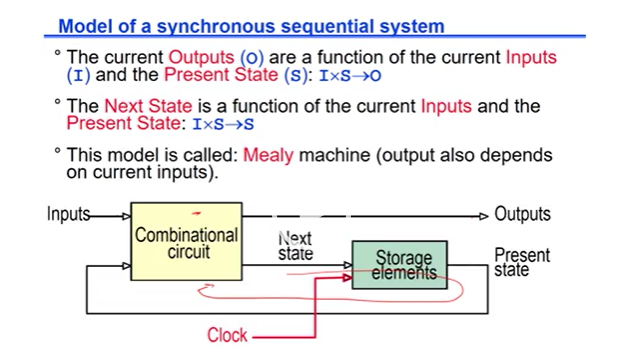
\includegraphics[width = \textwidth]{Pictures/Model of Synchronous Sequential Circuit.png}
    \caption{Basic Model}
\end{figure}
So we see, the next state passes through storage elements, and is not fedback directly into the system, which is synchronized with a clock.

\subsection{Flip-Flops}
\subsubsection{Use of FlipFlops}

\paragraph{Storing Data}
D Latch can not store data effectively:
\begin{figure}[H]
    \centering
    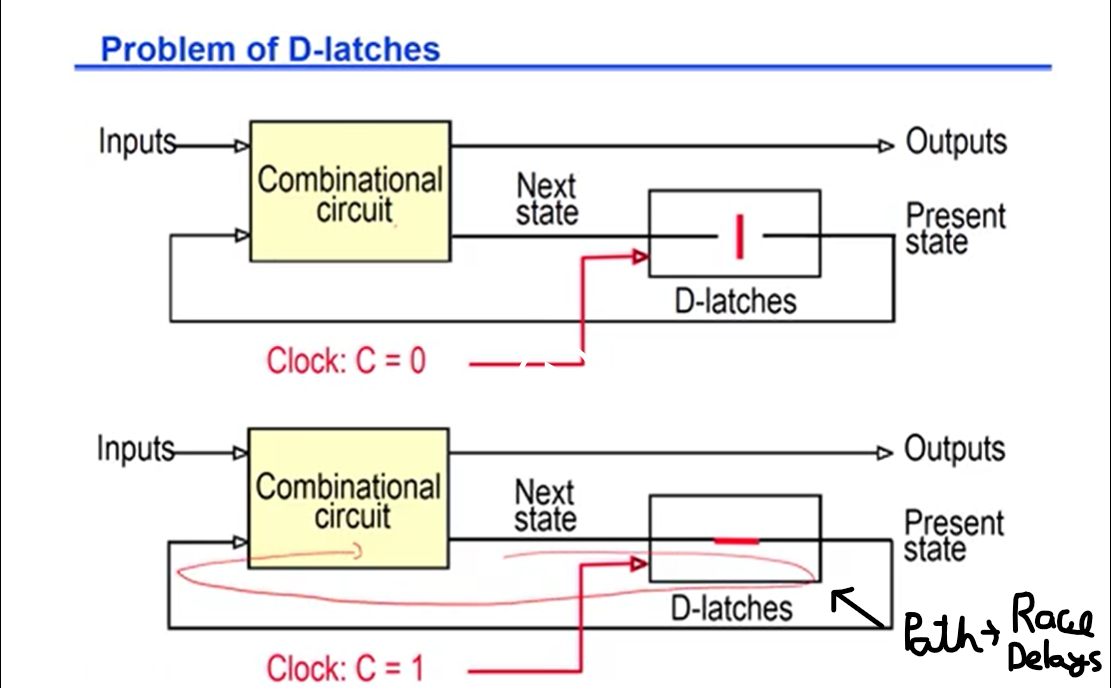
\includegraphics[width = \textwidth]{Pictures/Why Latches are not good for storing data.png}
    \caption{Creation of the combinatorial logic circuit, when C=1 means delays, race conditions and hence the fluctuations which end up changing the output, so storage not possible}
\end{figure}

Flip Flop:
\begin{figure}[H]
    \centering
    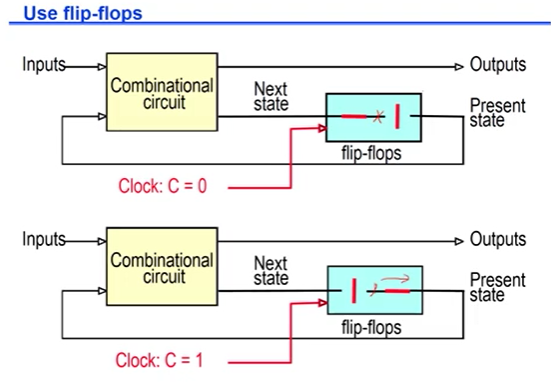
\includegraphics[width = \textwidth]{Pictures/Why Flip FLop good.png}
    \caption{Flip Flop good}
\end{figure}

\subsubsection{D-Flip Flop}
Q+ = D on active edge of the clock.
Q+ means after the active edge of the clock, not before not on.
\begin{enumerate}
    \item If Active Edge is rising edge, then triangle is uses,
    \item Else circle before the clock input is used.
\end{enumerate}
\begin{figure}[H]
    \centering
    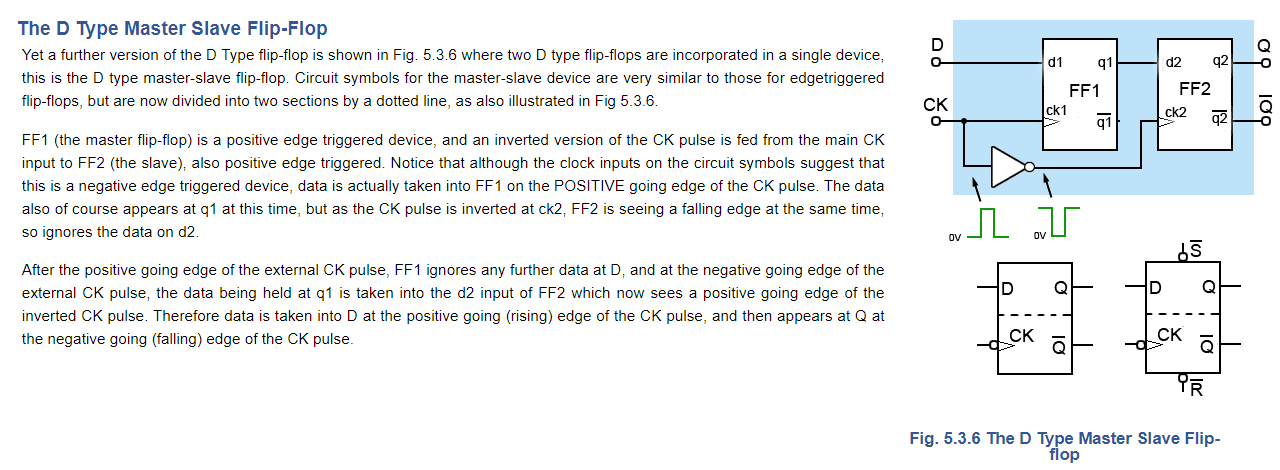
\includegraphics[width=\textwidth]{Pictures/D-FlipFlop.png}
    \caption{D-Flip Flop master-slave 1}
\end{figure}
\begin{figure}[H]
    \centering
    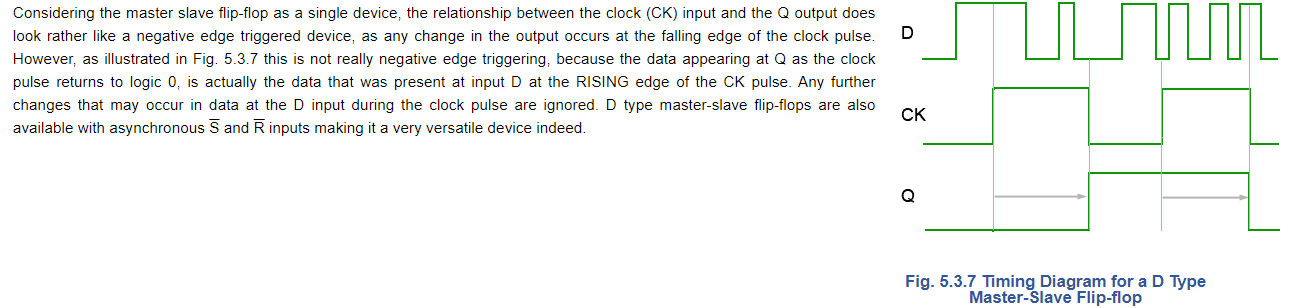
\includegraphics[width=\textwidth]{Pictures/D-FlipFlop2.png}
    \caption{D-Flip Flop master-slave 2}
\end{figure}
Click \href{https://learnabout-electronics.org/Digital/dig53.php}{Flip Flops} for more information.

\subsubsection{DE Flip Flop}
Same as D Flip Flop, but another input E, which determines if Q will change or not. If E=1, it is D Flip Flop, if E = 0, nothing happens.

\subsubsection{InitThe Flip Flop}
\begin{figure}[H]
    \centering
    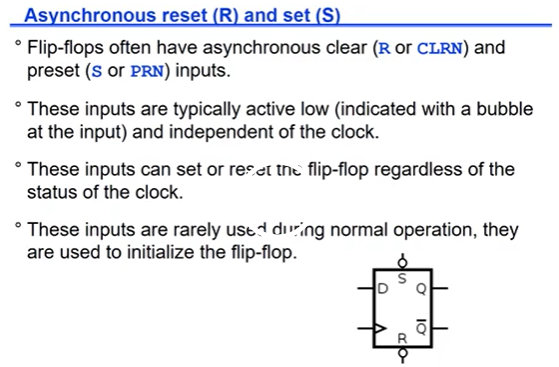
\includegraphics[width = \textwidth]{Pictures/Init the Flip Flop.png}
    \caption{The circle at S, R means when 0, then S=1, and vice-versa}
\end{figure}

\subsection{Timing}
\begin{figure}[H]
    \centering
    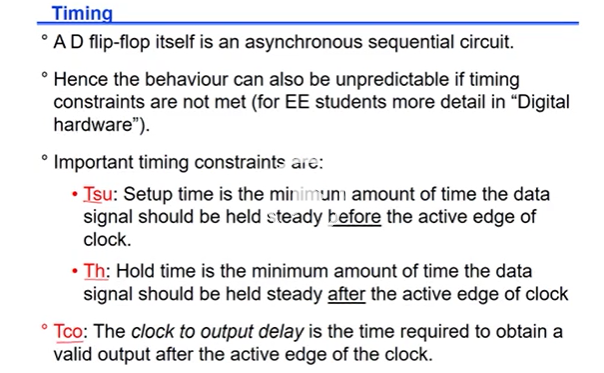
\includegraphics[width = \textwidth]{Pictures/Timing.png}
    \caption{The data should hold it's value, Tsu time before Active Edge and Th after active edge. The value in this time frame is copied.}
\end{figure}
\begin{figure}[H]
    \centering
    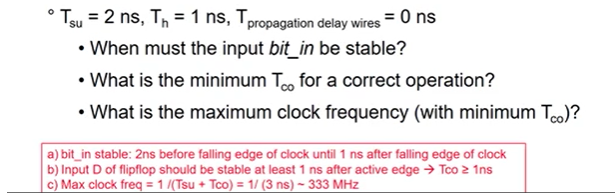
\includegraphics[width = \textwidth]{Pictures/Shift Reg Ex.png}
    \caption{Example of timing math}
\end{figure}

\section{Lecture 2}
\begin{enumerate}
    \item Design Synchronous Logic Circuits
    \item Analyse Synchronous Logic Circuits
\end{enumerate}

\subsection{Finite State Machines}
\subsubsection{Mealy Machines}
Mealy machine is a finite-state machine whose output values are determined both by its current state and the current inputs.\newline
A Mealy machine is a deterministic finite-state transducer: for each state and input, at most one transition is possible. There is one-to-one mapping.
 
 \begin{enumerate}
     \item Output depends on present state as well as present input.
     \item If input changes, output also changes.
     \item Less number of states are required.
     \item  There is more hardware requirement for circuit implementation.
     \item They react faster to inputs.
     \item Asynchronous output generation.
     \item Output is placed on transitions.
     \item It is difficult to design.
 \end{enumerate}
 
 \paragraph{Problem}
 \begin{figure}[H]
     \centering
     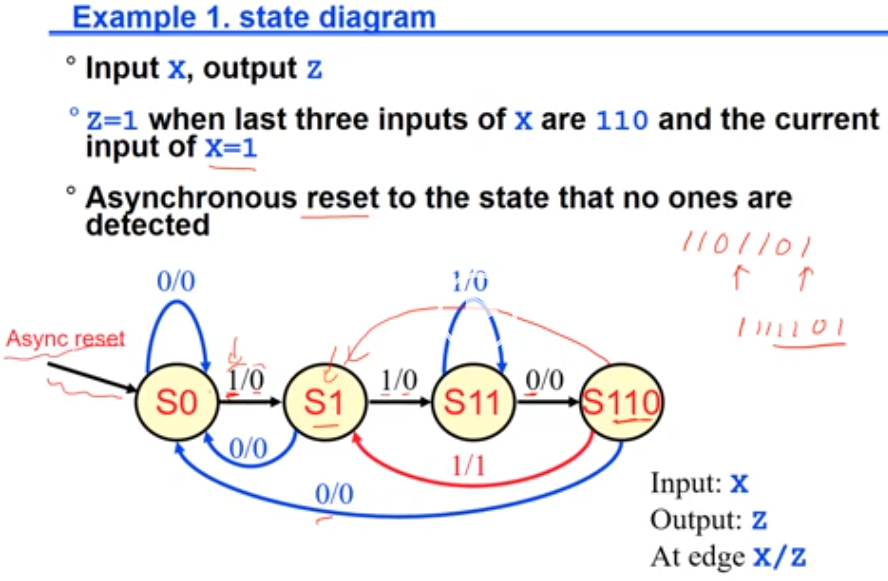
\includegraphics[width = \textwidth]{Pictures/FSM Ex1.png}
     \caption{Since Output depends on Input, this calls for a Mealy Machine. Use meaningful state names.}
 \end{figure}

\paragraph{Now convert this to a Sequential Logical Circuit\ Find SOP}
\begin{enumerate}
    \item Minimise the FSM (not part of the course, already is)
    \item Make a 2D non encoded truth table:
    \begin{figure}[H]
        \centering
        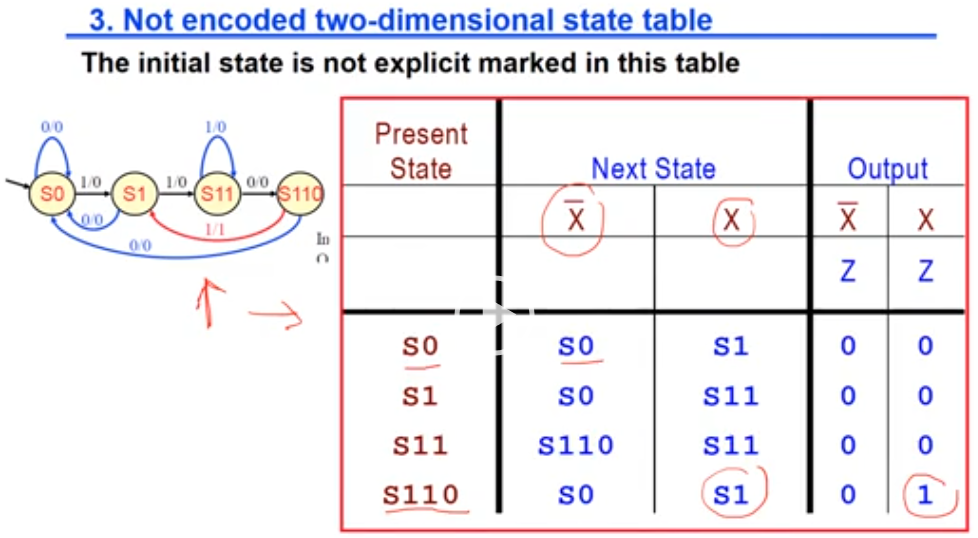
\includegraphics[width = \textwidth]{Pictures/FSM Ex1.1.png}
        \caption{2D non encoded truth table}
    \end{figure}
    \item Look at the number of states we have currently- 4. So how many bits we need? \textbf{Ans. 2}. To represent the entire range of 4 possible outputs we need at least 2 flip flops, since each flip holds one bit. So we get:
    \begin{figure}[H]
        \centering
        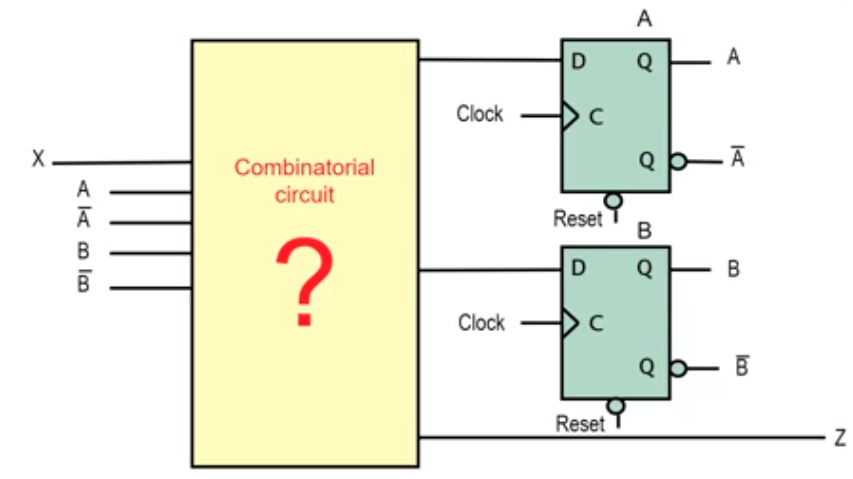
\includegraphics[width=\textwidth]{Pictures/FSM Ex1.3.png}
    \end{figure}
    Where A and B are:
    \begin{figure}[H]
        \centering
        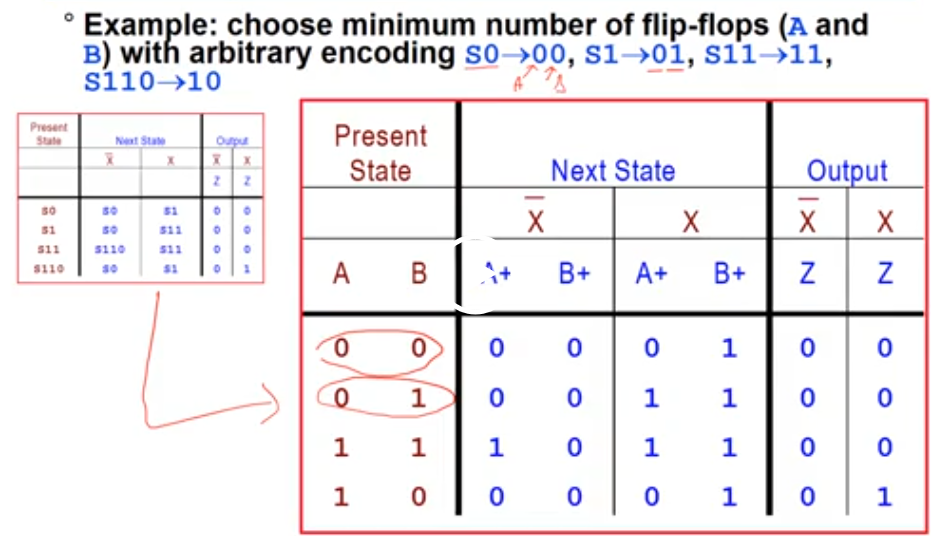
\includegraphics[width = \textwidth]{Pictures/FSM Ex1.4.png}
        \caption{Completed encoded table}
    \end{figure}
    \item Now to find the combinatorial logic, we need to reduce the 2D to 1D!.
    \begin{figure}[H]
        \centering
        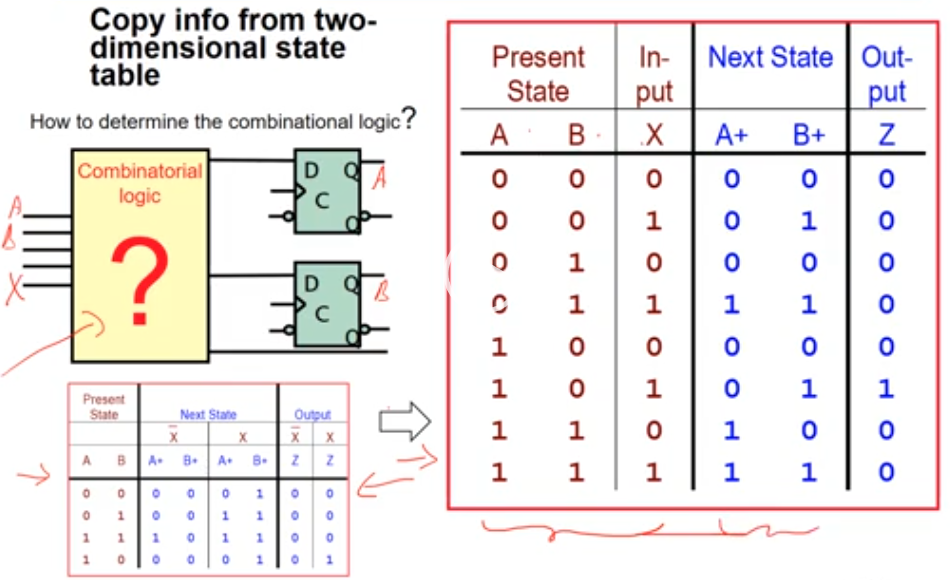
\includegraphics[width = \textwidth]{Pictures/FSM Ex1.5.png}
        \caption{The ABX colum reprsents the combinatorial logic}
        \item Normally we would choose a flip flop at this point, but in this course we only use D-FlipFlops so, we actually get the NextState in the table above to be the outputs of the Flip FLops 1 and 2. Notice the +, hence after the active edge of the clock.
        \item Get the logic:
        \begin{figure}[H]
            \centering
            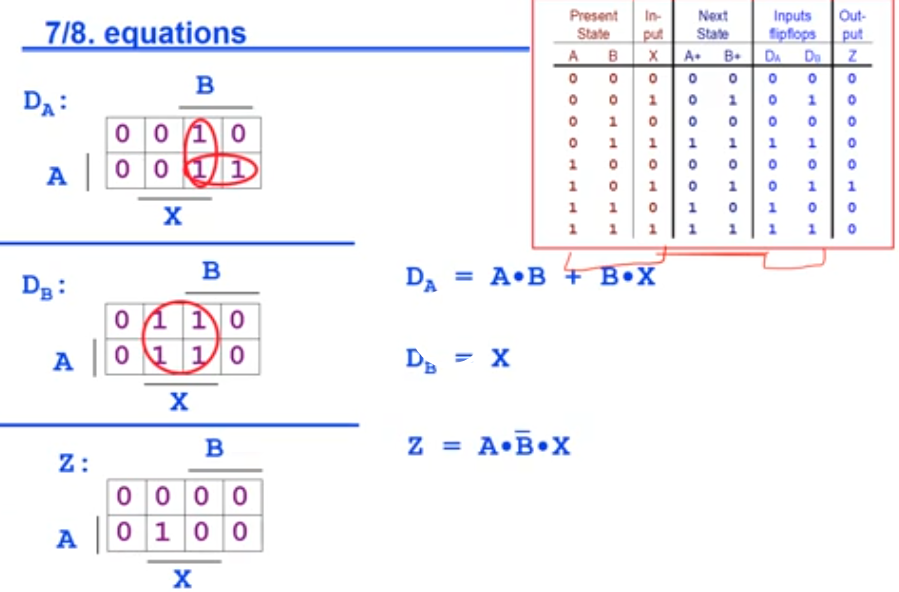
\includegraphics[width = \textwidth]{Pictures/FSM Ex1.6.png}
            \caption{Using Karnaugh Map}
        \end{figure}
    \end{figure}
    \item Finally draw it out:
    \begin{figure}[H]
        \centering
        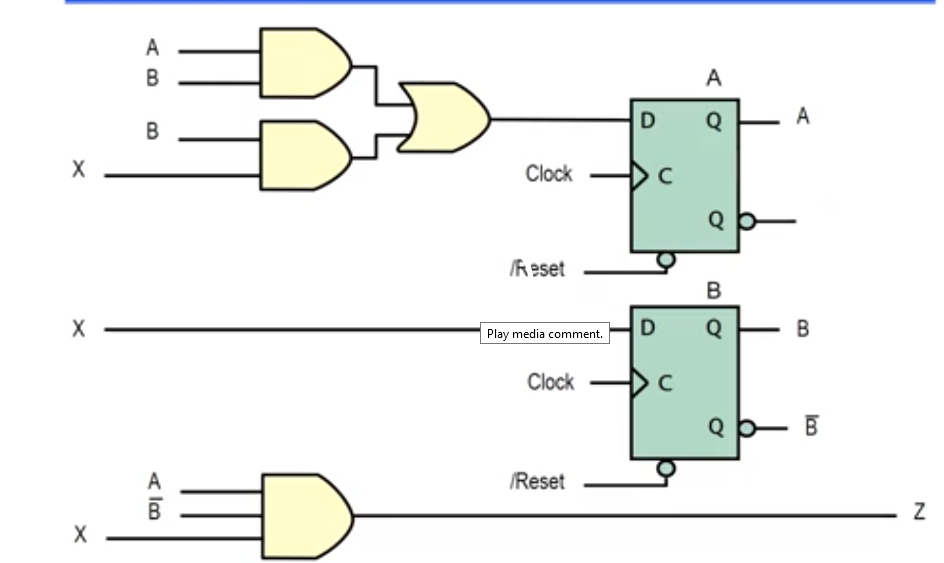
\includegraphics[width = \textwidth]{Pictures/FSM Ex1.7.png}
    \end{figure}
\end{enumerate}

\subsubsection{Moore Machine}
Moore machine, whose (Moore) output values are determined solely by its current state.

\begin{enumerate}
    \item Output depends only upon present state.
    \item If input changes, output does not change.
    \item More number of states are required.
    \item They react slower to inputs(One clock cycle later).
    \item There is less hardware requirement for circuit implementation.
    \item Synchronous output and state generation.
    \item Output is placed on states.
    \item Easy to design.
\end{enumerate}

\paragraph{Problem}
\begin{enumerate}
    \item Following the previous specification of the Mealy Machine:
    \item Input X, Output Z,
    \item Z=1, when last four inputs of X are 1101, notice how in mealy machine the as soon as the input becomes 1 after a 110, we get a 1, but in moore machine we will not get a 1 unless the state is in 1101 at the active edge of the clock.
\end{enumerate}
\paragraph{Convert this into a Circuit}

\begin{enumerate}
    \item 
    \begin{figure}[H]
        \centering
        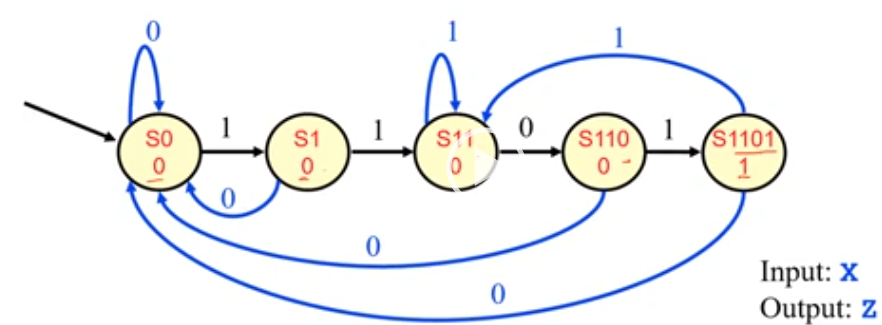
\includegraphics[width = \textwidth]{Pictures/FSM Ex2.png}
    \end{figure}
    \item From here the process is same as mealy. notice how we have 5 states, so not $2^{2}$, hence we need 3 flip flops instead.
    \item \textbf{HOLD UP:} one difference. Since output is dependant on state, the table as only output column.
    \begin{figure}[H]
        \centering
        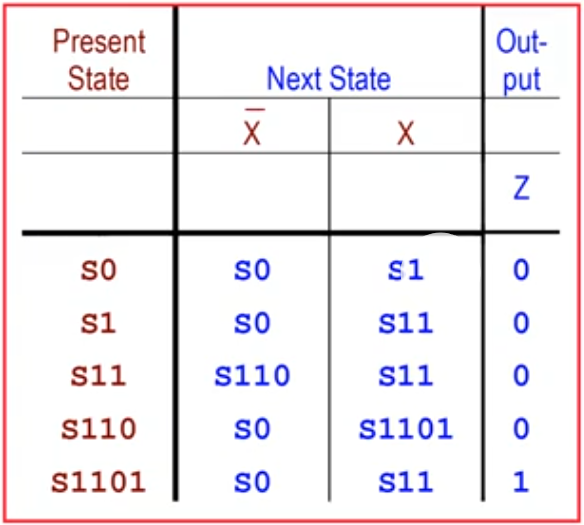
\includegraphics[width = 0.5\textwidth]{Module 5/Notes/Pictures/FSM Ex2.1.png}
    \end{figure}
    \item There can be unused state. This is okay. The unused state could be used for other states that we don't need to care about.
\end{enumerate}

\subsubsection{Reverse Process}
\paragraph{Problem}
\begin{figure}[H]
    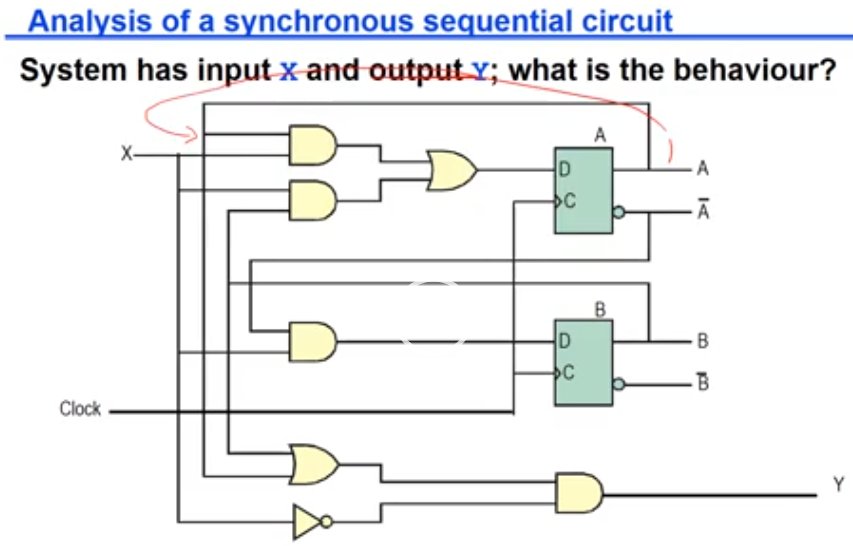
\includegraphics[width = 0.49\textwidth]{Pictures/FSM Ex3.png}
    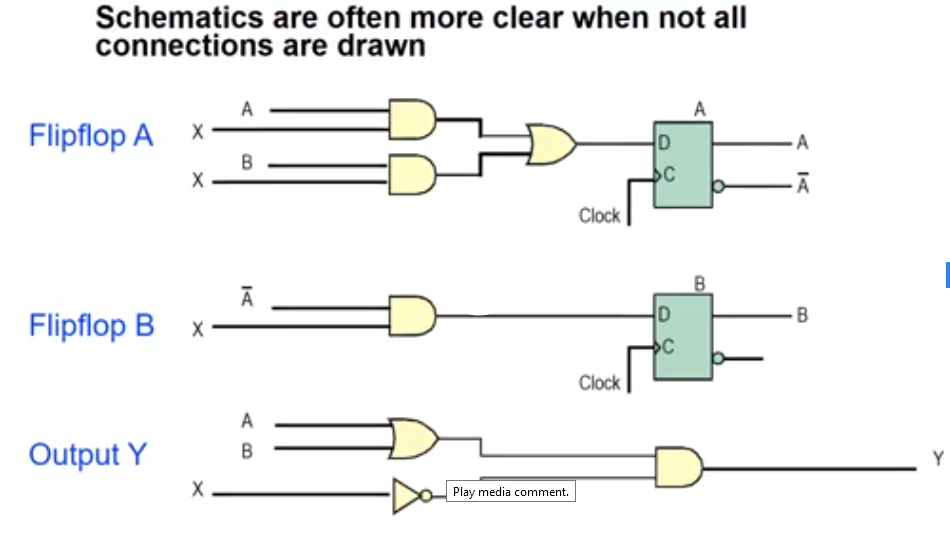
\includegraphics[width = 0.49\textwidth]{Pictures/FSM Ex3.1.png}
    \caption{It is easier to rewrite this into this:}
\end{figure}
\begin{enumerate}
    \item The Logics are:
    \begin{enumerate}
        \item $D_{A} = A.X + B.X$
        \item $D_{B} = \overline{A}.X$
        \item $Y = (A+B).\overline{X}$
    \end{enumerate}
    \item The 1D table and then Convert to 2D table splitting over values of X:
    \begin{figure}[H]
        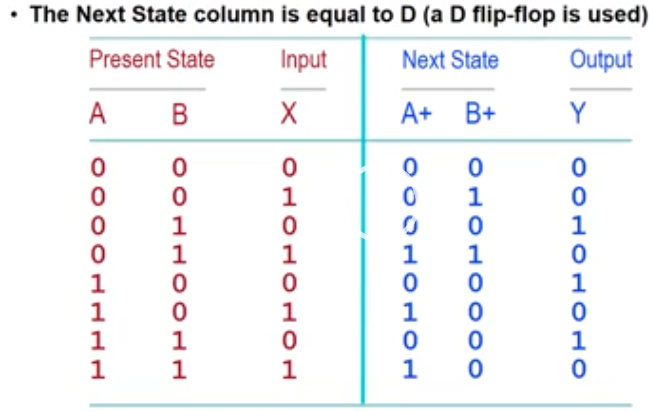
\includegraphics[width = 0.49\textwidth]{Pictures/FSM Ex3.2.png}
        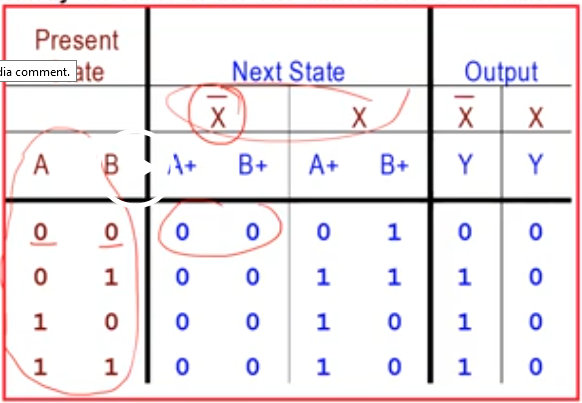
\includegraphics[width = 0.49\textwidth]{Pictures/FSM Ex3.3.png}
    \end{figure}
    \item Convert to Symbolic Names. and done.
    \begin{enumerate}
        \item $00 \to S0$
        \item $01 \to S1$
        \item $10 \to S2$
        \item $11 \to S3$
    \end{enumerate}
    \item Draw it out:
    \begin{figure}[H]
        \centering
        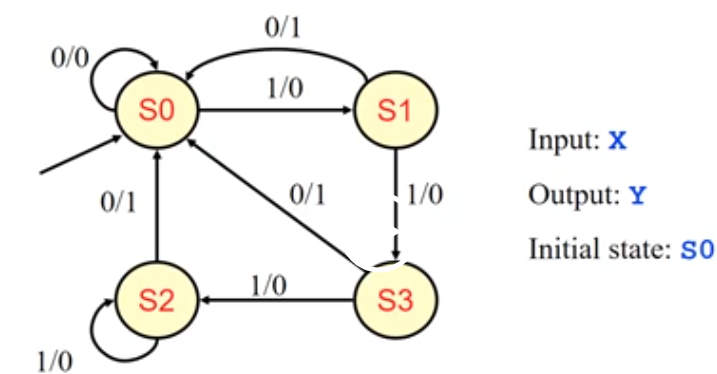
\includegraphics[width = \textwidth]{Pictures/FSM Ex3.4.png}
    \end{figure}
    \item This can be reduced, by using only S0 and S1, but that is not the main focus in this course.
\end{enumerate}

\section{Lecture 3}

We learn how to represent the following information in computer memory:
\begin{enumerate}
    \item Text
    \begin{enumerate}
        \item ASCII
        \item Unicode
    \end{enumerate}
    \item Numbers
    \begin{enumerate}
        \item BCD
        \item unsigned
        \item signed, sign and magnitude, 1's and 2's complement
        \item fixed point numbers
        \item floating point numbers
    \end{enumerate}
    \item A Computer Program
\end{enumerate}

\subsection{BCD- Binary Coded Decimal}
\begin{enumerate}
    \item The denary digits are represented using 4bit.
    \item represents only till 9
    \item needs correction of 0110 (or) 6 when addition resultin a digit being greater than 9.
    \item only 10 out 16 are used.
    \item Fixed point numbers can be represented exactly:
    $0.009 \to 0000 0000 0000 1001$
\end{enumerate}

\subsection{Different Base Sytems}
\subsubsection{base 2- Binary}
\paragraph{Denary to Binary}
\begin{enumerate}
    \item Number: 90
    \item 90 \% 2 = 0
    \item 45 \% 2 = 1
    \item 22 \% 2 = 0
    \item 11 \% 2 = 1
    \item  5 \% 2 = 1
    \item  2 \% 2 = 0
    \item  1 \% 2 = 1
    \item  0 \% 2 = 0
    \item following only 0 now
    \item Read the upper down to up: \textbf{01011010}
\end{enumerate}
\paragraph{What about Decimal}
\begin{enumerate}
    \item \textbf{Number: 0.5}
    \item $2^{-1} = 0.5$
    \item $0.5_{\{10\}} = (0.1)_{\{2\}}$
    \item \textbf{Number: 0.4}
    \item 0.4 - 0.25 = 0.15 ($2^{-2}$)
    \item 0.15 - 0.125 = 0.025 ($2^{-3}$)
    \item and so on....
    \item \textbf{Better way:}
    \item 0.4*2 = \textbf{0}.8
    \item 0.8*2 = \textbf{1}.6
    \item 0.6*2 = \textbf{1}.2
    \item 0.2*2 and so one, deducting 1 if over one for the next multiplication
    \item Read it top to bottom: \textbf{$(0.011)_{\{2\}}$}
\end{enumerate}
\subsubsection{base 8- Octal}
Above with 8
\subsubsection{base 16- Hexadecimal}
after 9: A,B,C,D,E,F
Above with 16
\subsubsection{All others are also possible 7, 9, 11, etc}
Extend with alphabets as needed,
Above with n
\subsection{Negative Numbers}
\subsubsection{Sign and Magnitude}
\begin{enumerate}
    \item MSB = Sign Bit
    \item rest N-1 bits = Value
    \item 1 is negative
    \item 0 is positive
    \item Two representation of 0 (We do not like this): 00, 10
    \item straight forward conversion
\end{enumerate}
\begin{equation}
    V = (-1)^{b_{N-1}}*\sum_{i=0}^{N-2}(b_{i}*2^{i})
\end{equation}
\subsubsection{1s Complement}
\begin{enumerate}
    \item MSB = Sign bit
    \item 1 is negative
    \item 0 is positive
    \item is Signed bit is set, the N-1 bits after MSB are flipped.
    \item two representation of zero: 00, 11
    \item for positive it is the same,
    \item for negative write the positive one, then flip all bits
    \item Ex: $-3 => 3 = 0011$, $ -3 = 1100$
    \item Arithmetic: end around carry
    \begin{enumerate}
        \item -1 + 2 = 1
        \item 110 + 010 = 1000
        \item 000 + 001 (take the carry and add it to back) = 001 = 1
    \end{enumerate}
\end{enumerate}
\begin{equation}
    V = (-1)^{b_{N-1}}*\sum_{i=0}^{N-1}(b_{i}*2^{i})
\end{equation}
\subsubsection{2s Complement}
\begin{enumerate}
    \item 1 is negative
    \item 0 is positive
    \item We can represent one extra negative number than positive numbers
    \item Same hardware can be used add unsingned and 2s complement numbers.
    \item
    \begin{equation}
        V = (-1)*({b_{N-1}}*2^{N-1})+\sum_{i=0}^{N-1}(b_{i}*2^{i})
    \end{equation}
    \item Conversion:
    \begin{enumerate}
        \item make into 1s
        \item add 1
        \item 5 = 0101
        \item -5 = 1010 (1s)
        \item -5 = 1011 (2s)
    \end{enumerate}
    \item The carry is thrown in arithmatic, if the number is range of the number of bits used. If number goes beyond, we get overflow errors.
\end{enumerate}
\subsubsection{Excess or Biased}
\begin{enumerate}
    \item excess -N means new V = V - N
    \item 0 = 000, now excess 3 means = 0 - 3 = -3 = 101
    \item a correction needs to be applied during arithmetic:
    \begin{enumerate}
        \item a -b + c -b = a+c -2b
        \item Linear Algebra: translation is not linear, so correction of +b during adding and -b during subtraction
    \end{enumerate}
    \item \textbf{When stored we add excess, when reading mme minus excess}
\end{enumerate}
\subsection{Fixed Point Representation}
\begin{enumerate}
    \item P is the position of the point from the right.
    \item So, multiply the whole binary representation with $2^{-P}$ to get the result
\end{enumerate}
\subsection{Floating Point Representation}
\subsubsection{Exponent and Mantissa}
\begin{enumerate}
    \item Mantissa is the M in $M * B^{E}$
    \item E is the power to which the base B is raised to in in $M * B^{E}$
    \item increasing size of mantissa increases precision
    \item increasing size of exponents increases range
    \item changing the size of exponent and mantissa changes the range and precision of the binary representation
\end{enumerate}
\subsubsection{Normalisation}
\begin{enumerate}
    \item 20E2 = 2E3, in storing numbers we would like to avoid this same number different representation, imagine 200 $\neq$ 200 in program code. Can you imagine.
    \item Normalise it.
    \item for every shift in the Mantissa increase or decrease exponent value.
    \item 0100.E0110 = 4E6
    \item 0.1E0111 = 0.5E9, this is normalised
    \item if negative:
    \item 1001.E0110 = -7E6
    \item 1.001E = -0.7E9
    \item so shift till the first 1 or 0, right of 1 if negative number, left of one if positive (as shown above, don't mix your right, his left stuff, I don't get that)
    \item in practice since the first bit is always 1, we dont store that bit, it is called hidden bit, hence we can one more order of precision/range stored.
\end{enumerate}
\begin{figure}[H]
    \centering
    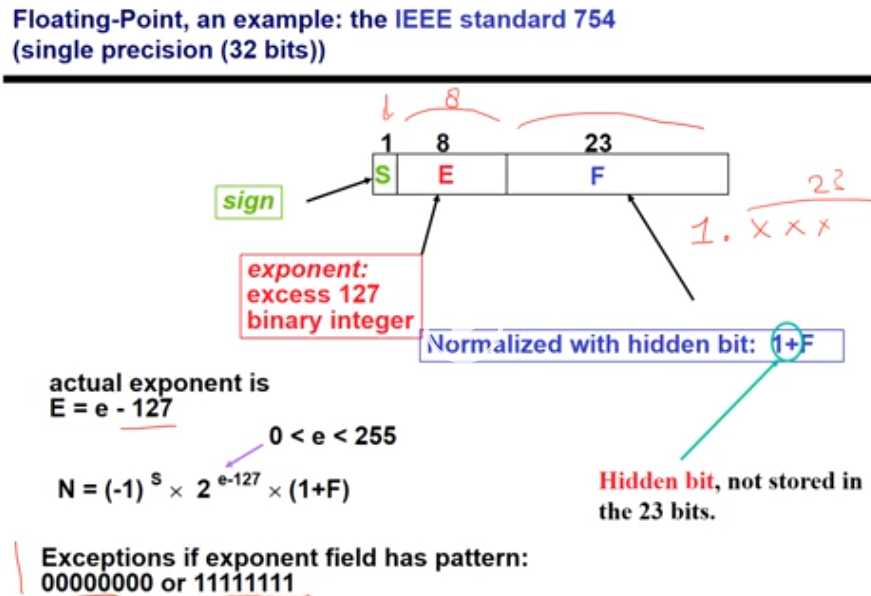
\includegraphics[width = \textwidth]{Module 5/Notes/Pictures/Floating Point Standard.png}
    \caption{An example in real Life}
\end{figure}

\subsubsection{Examples}
\paragraph{E: bits, Excess: 20, M:6 (excluding hidden), B:2}
\begin{enumerate}
    \item 1 01110 010000
    \begin{enumerate}
        \item sign = 1
        \item E = e-20 = 14-20 = -6
        \item M = 1.010000 = 1.25
        \item Result: -1.25E-6
    \end{enumerate}
    \item 4.75
    \begin{enumerate}
        \item 4.75 = 0100.11
        \item sign = 0
        \item e = E + 20 = 2 + 20 = 22 = 10110
        \item M = 1.0011 = 001100 (remove the hidden bit)
        \item res = 0 10110 001100
    \end{enumerate}
    \item 2.30
    \begin{enumerate}
        \item 2.30 = 010.01001100110011001100110011
        \item sign = 0
        \item e = E + 20 = 1 + 20 = 21 = 10101
        \item M = 1.00100110011 = 001001 (remove hidden bit)
        \item res = 0 10101 001001
    \end{enumerate}
\end{enumerate}

\subsubsection{IEEE 754- single precision}
\begin{enumerate}
    \item Sign Bit 1
    \item Mantissa 24
    \item Exponent 8bits 127 excess
    \item Special Numbers:
    \begin{figure}[H]
        \centering
        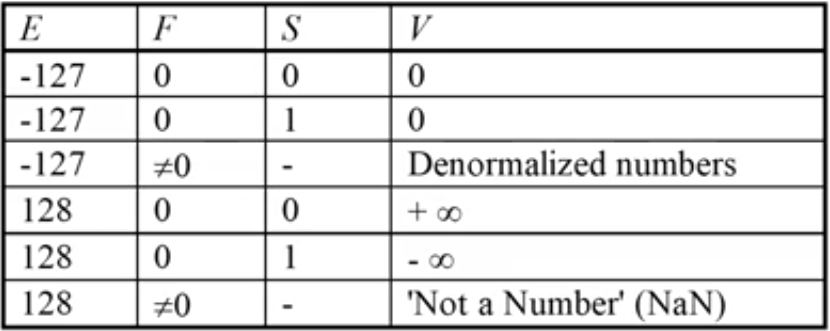
\includegraphics[width=\textwidth]{Module 5/Notes/Pictures/IEEE754SinglePrecisionSpecialNumbers.png}
    \end{figure}
\end{enumerate}

\section{Lecture 4}
\subsection{Signed and Unsigned Addition}
\subsubsection{Unsigned Number}
\begin{enumerate}
    \item Same as decimal addition.
    \item In case of overflow, number can not be represented.
\end{enumerate}
\subsubsection{Full Adder/Ripple Carry Adder}
\begin{enumerate}
    \item CarryIn
    \item inA and inB
    \item SumOut
    \item Carry Out
    \item We can use Karnaugh Map to find Logic of SumOut and CarryOut with the three inputs.
    \item Delay: $N*2\delta$ where $2\delta$ is the delay of one adder, so N bit adder have N times.
\end{enumerate}
\subsubsection{Signed Numbers}
\begin{enumerate}
    \item MSB has negative weight
    \begin{enumerate}
        \item So, 011+110 = 3 - 2 = 1
        \item but adding also gives the same since Carry is positive 1 not negative weight.
    \end{enumerate}
    \item Can use FA, where final carry out is ignored.
\end{enumerate}
\subsubsection{Overflows}
\begin{enumerate}
    \item A positive number and negative number can never result in overflow.
    \item Only both positive or both negative numbers can.
\end{enumerate}
\subsubsection{Detecting Overflows}
\begin{enumerate}
    \item Using Karnaugh Map and finsind logic.
    \item Sign Bit Extension
    \begin{figure}[H]
        \centering
        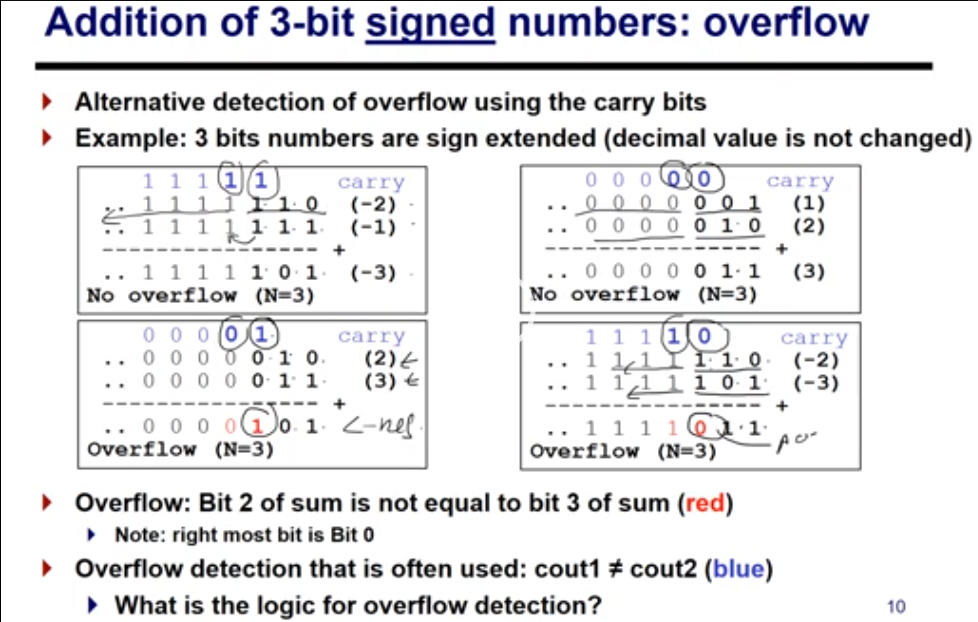
\includegraphics[width = \textwidth]{Module 5/Notes/Pictures/Overflow Detection.png}
    \end{figure}
\end{enumerate}
\subsubsection{Adding Different Length}
\begin{enumerate}
    \item Sign Extend shortest operand
\end{enumerate}
\subsubsection{Addition and Subtraction using FA}
\begin{enumerate}
    \item XOR the bits with mode, and set $C_{0}$ to the mode where 0 is addition and 1 is subtraction.
\end{enumerate}
\subsection{How computers use this for programs}
\subsubsection{Status bits}
\begin{enumerate}
    \item N - negative: The output of final SOut
    \item V - Overflow: XOR of last two carry bits
    \item Z - Zero: NOR all SOuts
    \item C - Carry: The final Carry Out
\end{enumerate}
\subsection{Unsigned Multiplcation}
\subsubsection{In process}
\begin{enumerate}
    \item It easy, just remember that multiplying by two shifts the bits to the left, similarly dividing by 2 shifts bits to right.
    \item but What about hardware?
\end{enumerate}
\subsubsection{In Hardware}
\begin{enumerate}
    \item Shift Add Algorithm \textbf{Combinatorial}
    \begin{figure}[H]
        \centering
        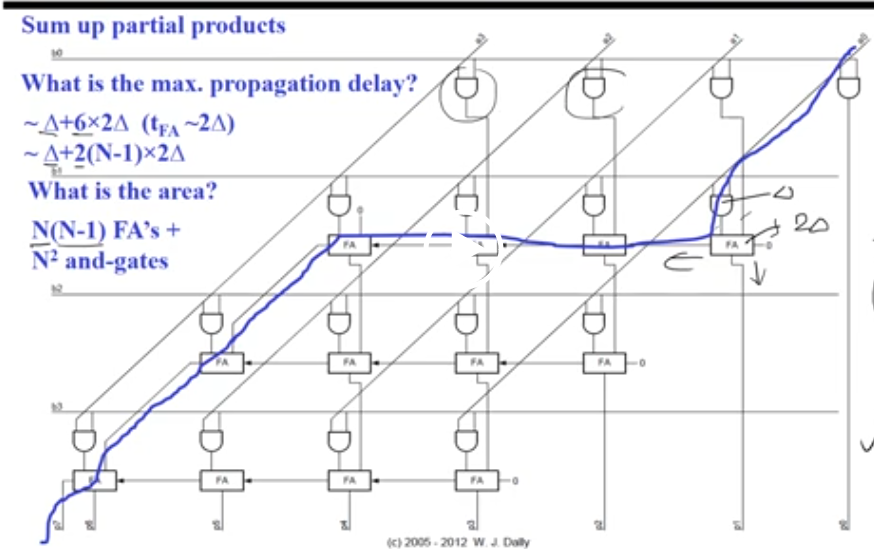
\includegraphics[width = \textwidth]{Module 5/Notes/Pictures/Shift-Add.png}
    \end{figure}
    \item Shift Add Algorithm \textbf{Sequential}
    \begin{figure}[H]
        \centering
        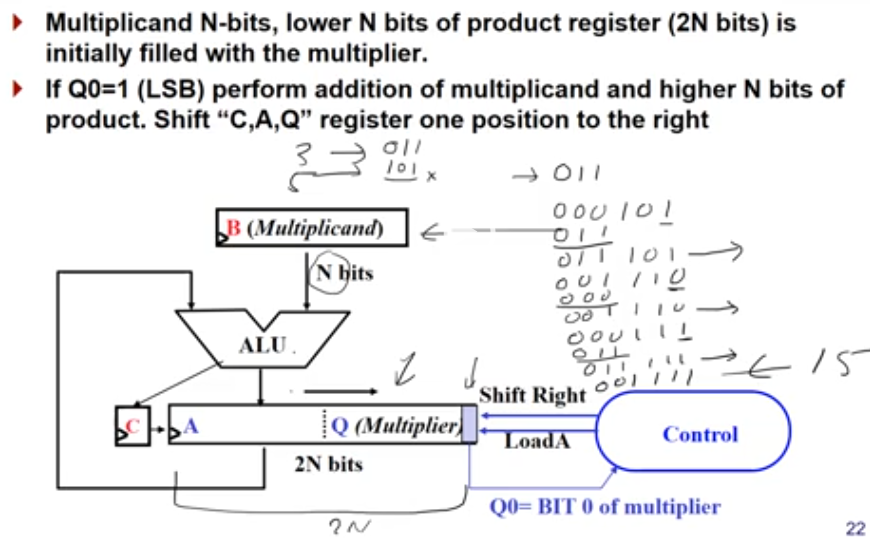
\includegraphics[width = \textwidth]{Module 5/Notes/Pictures/Sequetial Mul.png}
        \caption{Clock Cycles = 1 + 2*N, where N is the number of bits and 1 is for init}
    \end{figure}
\end{enumerate}
\subsubsection{Signed Multiplication}
\textbf{Not part of CAO for TCS}
\subsection{Processor}
\begin{figure}[H]
    \centering
    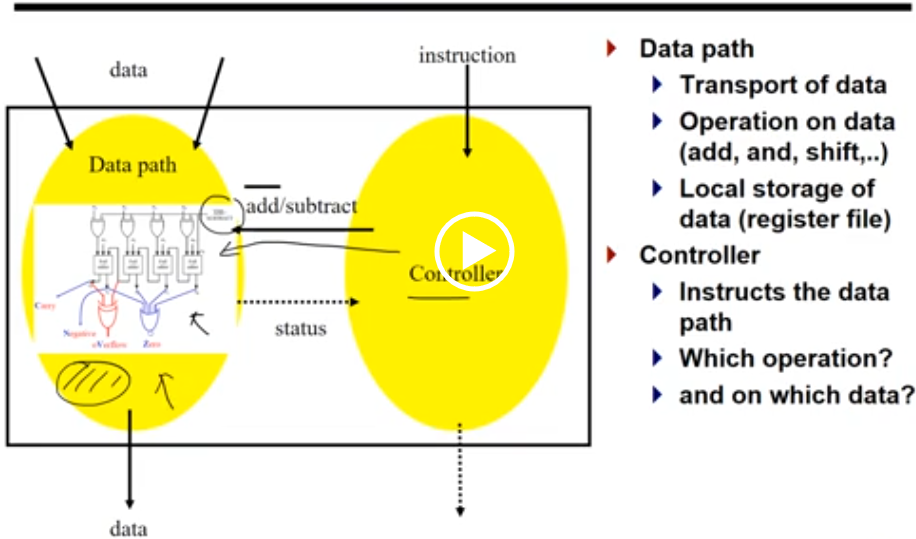
\includegraphics[width = \textwidth]{Module 5/Notes/Pictures/Incomplete Simple Processor.png}
\end{figure}
\subsubsection{Parts}
\paragraph{Data Path}
\begin{enumerate}
    \item ALU
    \item Buses
    \item Multiplexors
    \item Registers
\end{enumerate}
\paragraph{Controller}
\begin{enumerate}
    \item Function
    \begin{enumerate}
        \item Determines What Operation
        \item Receives Status Information from datapth
    \end{enumerate}
    \item Types
    \begin{enumerate}
        \item Hard Wired (FSM)
        \item Micro-Programmed (More Flexible)
        \begin{figure}[H]
            \centering
            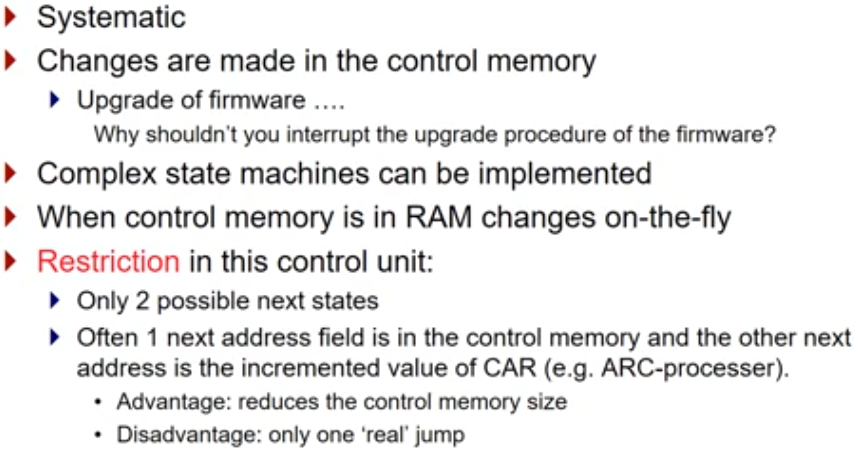
\includegraphics[width = \textwidth]{Module 5/Notes/Pictures/Advantages of Micro-Programming.png}
        \end{figure}
    \end{enumerate}
\end{enumerate}
\paragraph{Registers}
\begin{figure}[H]
    \centering
    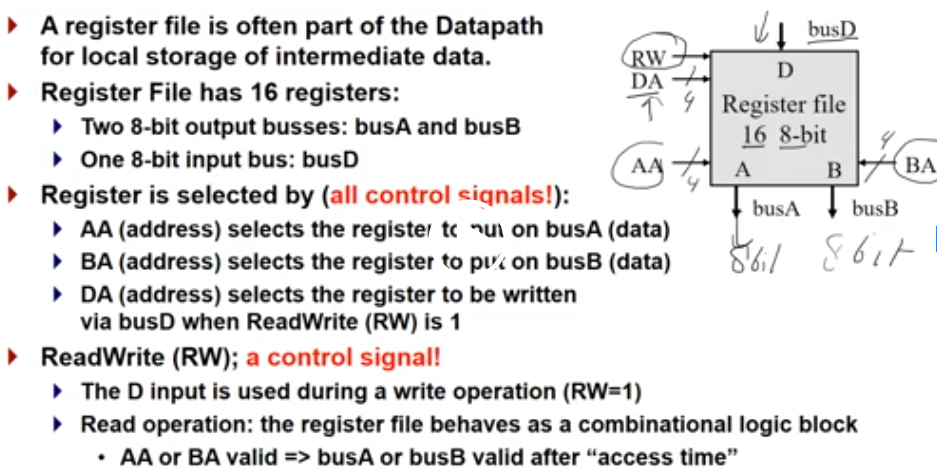
\includegraphics[width = \textwidth]{Module 5/Notes/Pictures/Register File.png}
\end{figure}
\paragraph{Shifter}
\begin{figure}[H]
    \centering
    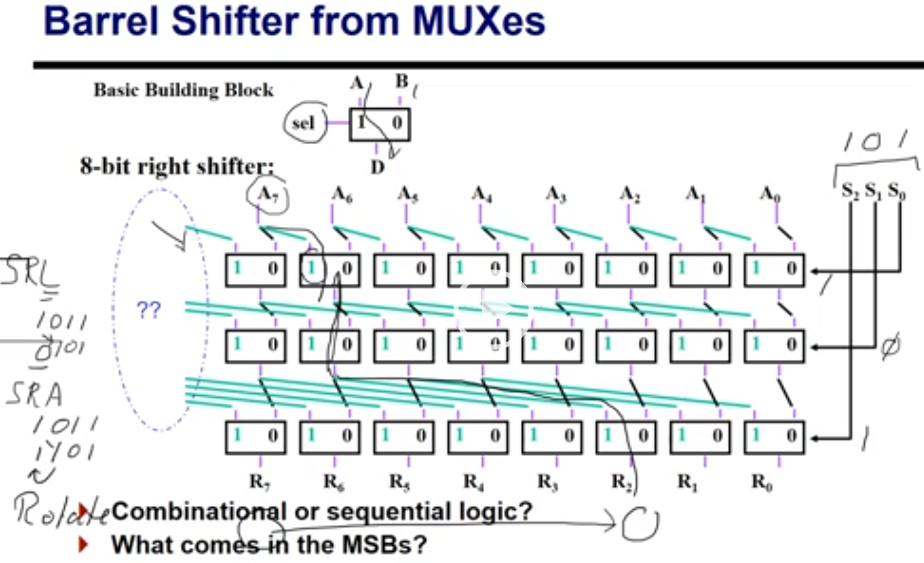
\includegraphics[width = \textwidth]{Module 5/Notes/Pictures/Barrel Shifter.png}
\end{figure}

\section{Lecture 5}
\subsection{Stack}
\begin{enumerate}
    \item LiFO
    \item POP, PUSH
    \item Most processors have a special stack pointer
    \item Where does the pointer point?
    \begin{enumerate}
        \item Last Occupied or next free?
        \item Last Full
        \begin{enumerate}
            \item SP += 1
            \item Mem[SP] = Reg
        \end{enumerate}
        \item Next Empty
        \begin{enumerate}
            \item Mem[SP] = Reg
            \item SP += 1
        \end{enumerate}
    \end{enumerate}
    \item How does Stack grow?
    \begin{enumerate}
        \item Small to Big
        \begin{enumerate}
            \item always
        \end{enumerate}
    \end{enumerate}
\end{enumerate}

\subsection{ISA}
\begin{figure}[H]
    \centering
    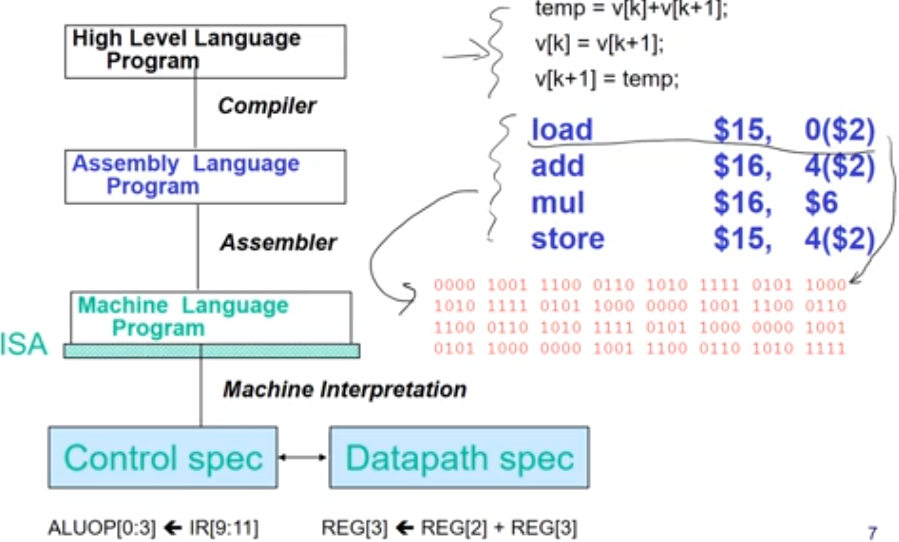
\includegraphics[width = \textwidth]{Module 5/Notes/ISA.png}
\end{figure}
\subsubsection{Fetch Execute Cycle}
\begin{enumerate}
    \item Fetch
    \begin{enumerate}
        \item From Registers
    \end{enumerate}
    \item Decode
    \item Operand
    \begin{enumerate}
        \item From GPR (General Purpose Registers)
        \item Also use ACC (Accumulator)
    \end{enumerate}
    \item Execute/Store
    \begin{enumerate}
        \item In Memory
        \item Display on computer (any I/O)
    \end{enumerate}
    \item Next
    \begin{enumerate}
        \item Using PC (Program Counter)
    \end{enumerate}
\end{enumerate}

\subsubsection{RPN- Calculation using Stack}
\begin{enumerate}
    \item Find relation put write togethor ending with relation
    \item $\frac{2+7}{3} + (100 * 9)$
    \item res = 2 5 + 3 / 100 9 * +
    \begin{enumerate}
        \item store 2
        \item store 7
        \item add
        \item store 3
        \item divide by 3 and store into stack
        \item store 100
        \item store 9
        \item multiply 100 and 9 and store
        \item add last two entries on stack
        \item output result = 903
    \end{enumerate}
\end{enumerate}

\subsubsection{Endianess}
\begin{enumerate}
    \item If value read into memory left to right, then big endianess, so the first char has the lowest address in a stack.
    \item if value read into memory right to left, then small endianess, so the first char has the highest address in  a stack.
\end{enumerate}

\subsubsection{Aligned Memory}
\begin{enumerate}
    \item Use the same leading bits for first n-m bits where m < n, then we can access m memory cells at the same time to get all bits of the data split over these memory cells.
\end{enumerate}

\subsubsection{CISC and RISC}
\paragraph{CISC}
Complex Instruction Set Computer

\begin{enumerate}
    \item Code Size is prioritised:
    \begin{enumerate}
        \item Variable length codes
        \item hardware dependant
        \item variable clock cycles
        \item can perform complex tasks
        \item Many addressing modes
    \end{enumerate}
\end{enumerate}

\paragraph{RISC}
Reduced Instruction Computer
    \begin{enumerate}
        \item Constant length codes
        \item software dependant
        \item 1 clock cycle length tasks
        \item can perform simple tasks only
        \item Simple addressing Mode
    \end{enumerate}

\section{Lecture 6 (and 5) ARC pointers}

\begin{enumerate}
    \item Not bytes, words
    \item bit 13
    \item simm13 - gives lower 13 bits
    \item sethi needs to be followed by or or +
    \item jumpl pc+4, r0
    \item orn
    \item 1 (op) (op3) 00
    \item rtl instructions, fetch decode then
\end{enumerate}

\section{Lecture 7}
\subsection{Levels of Computer}
\begin{enumerate}
    \item Architecture: Registers, micro-controlled processor, etc
    \item Organisation: Timing
    \item Physical: Wires, transistors
\end{enumerate}

\subsection{Definition}
\begin{enumerate}
    \item Bit: 1
    \item Nibble: 4
    \item Byte: 8
    \item Half Word: 16
    \item Word: 32
    \item double: 64
    \item quad: 128
\end{enumerate}

\subsection{Important Concepts}
\subsubsection{Moore's Law}
\subsubsection{Von Neuman Architecture}
\paragraph{Has 5 Units}
\begin{enumerate}
    \item ALU
    \item Input Unit
    \item Output Unit
    \item Memory Unit (for intermeddiate calculations)
    \item Control Unit
\end{enumerate}

\paragraph{A refinement}
\begin{enumerate}
    \item CPU
    \item memory
    \item I/O unit
    \item Buses:
    \begin{enumerate}
        \item Data
        \item Control
        \item Address
        \item Power
        \item Possibly I/O bus
    \end{enumerate}
\end{enumerate}

\subsection{What is Bus?}
\begin{enumerate}
    \item A communication pathway connecting two or more devices
    \item Often grouped to form system bus width
    \item They are broadcast
\end{enumerate}
\paragraph{Data Bus}
Transports data and instructions \\
Data Bus width is key to performance


\paragraph{Address Bus}
Identifies the source or the destination, for ex. when CPU needs to read from the memory
Address bus determines the maximum memory capacity of the system, i.e. the number of possible addressable places in RAM.

\paragraph{Control Bus}
\begin{enumerate}
    \item Control and timing information
    \begin{enumerate}
        \item Memory read write
        \item Interrupt Requests
        \item Clock Signals
    \end{enumerate}
\end{enumerate}

\subsubsection{Addressing}
\begin{enumerate}
    \item Involves all 3 buses
    \begin{enumerate}
        \item If want to access a memory location
        \item Address Bus gives address
        \item Data bus tells you the data, or writes
        \item depending on the clock sync and information by controller.
    \end{enumerate}
    \item Uses the conventions of alignment
    \begin{enumerate}
        \item Use capacity of the data bus, as much as possible
        \item So, if word is 32bits, for a given address we ignmore last 2 bits, and transport the 4 bytes.
    \end{enumerate}
    \item Thing to remember
    \begin{enumerate}
        \item Since we address the whole 32 bits, even if we want to store in a particular location, we end up overwriting the other 3 bytes, in case of storing exactly 8 bits. While writing. So we add BE flags byte enabled, to set all other vytes in the block to 0, and the active block to 1.
        \item The processor will need to extract the correct path while reading data.
    \end{enumerate}
\end{enumerate}

\end{document}
